%%%%%%%%%%%%%%%%%%%%%%%%%%%%%%%%%%%%%%%%%%%%%%%%%%%%%%%%%%%%%%%%%%%%%%%%%%%%%%%%
% INSTRUCTIONS
% - please add any additional references to additional.bib, NOT SymbolicRegression.bib
%%%%%%%%%%%%%%%%%%%%%%%%%%%%%%%%%%%%%%%%%%%%%%%%%%%%%%%%%%%%%%%%%%%%%%%%%%%%%%%%
\section{Introduction}
%%%%%%%%%%%%%%%%%%%%%%%%%%%%%%%%%%%%%%%%%%%%%%%%%%%%%%%%%%%%%%%%%%%%%%%%%%%%%%%%

%In regression analysis, symbolic regression stands out as an approach that searches for a mathematical expression describing the input-output relationship of the studied phenomena. It differs from most regression models since it does not part from a fixed structure, thus having the possibility of finding a simpler expression.

Symbolic regression (SR) is an approach to machine learning (ML) in which both the parameters and structure of an analytical model are optimized. 
SR can be useful when one wishes to describe a process via a mathematical expression, especially a simple expression; thus, it is often applied in the hopes of producing a model of a process that, by virtue of its simplicity, may be easy to interpret.

SR literature has, in general, fallen short of evaluating and/or identifying any method or family of methods that could be considered ``state-of-the-art'' (SotA).
In large part, these shortcomings are due to longstanding issues with the datasets used to benchmark symbolic regression, which are often small, trivial, or simply not standardized (i.e. comparable) across papers or experiments~\cite{mcdermottGeneticProgrammingNeeds2012b}.

Although community surveys~\cite{whiteBetterGPBenchmarks2012a,mcdermottGeneticProgrammingNeeds2012b} have led to suggestions for improving benchmarking standards, and even black-listed certain problems, contemporary literature continues to be published that partly violates those standards~\cite{petersenDeepSymbolicRegression2020}.
Furthermore, there is a lack of cross-pollination between the research communities interested in symbolic regression, which include evolutionary computation, physics, engineering, statistics, and more traditional machine learning disciplines. 
Finally, lack of consensus on what SR methods constitute ``SotA'' is due in part to the ways in which methodological studies may be conducted - i.e., the relative merit of conducting incremental ablation studies versus large benchmark studies, such as this one. 
Whatever the causes, the result is that promising directions for future research in symbolic regression are not well-informed by empirical evidence. 

The aspects of performance assessment for symbolic regression differ from typical regression benchmarking due to the interest in obtaining concise, symbolic expressions. 
In general, the trade-off between accuracy and simplicity must be considered when evaluating the merits of different models.  
Furthermore, model \emph{simplicity}, typically measured as sparsity or model size, is but a proxy for model \emph{interpretability}; a simple model may still be un-interpretable, or simply wrong~\cite{liptonMythos2018,poursabziManipulating2021,virgolinModelLearning2021}. 
With these concerns in mind, datasets with ground truth solutions are useful, in that they allow researchers to assess whether or not the symbolic model regressed by a given method corresponds to a known analytical solution. 
Assessing whether the symbolic model returned by a model is an exact match is non-trivial, and requires symbolic solvers equipped with a combination of algebraic simplification and structural pruning techniques.
In addition, relative fidelity of estimated model forms that are not exact matches are difficult to assess.

As synthetic datasets with ground truth solutions are not sufficient for benchmarking symbolic regression algorithms, we consider it essential to also evaluate the performance of SR on real-world or otherwise black-box regression problems, relative to SotA ML methods. 


%Such datasets do not give an adequate view into the expected performance of the algorithm when applied to datasets whose forms are yet to be discovered. 

In this paper, we describe a large benchmarking effort that includes a dataset repository curated for symbolic regression, as well as a benchmarking library designed to allow methodologists to easily contribute methods. 
To achieve this, we incorporated 130 datasets with ground truth forms into the Penn Machine Learning Benchmark (PMLB)~\cite{olsonPMLBLargeBenchmark2017d}, including metadata describing the underlying equations, their units, and various summary statistics. 
Furthermore, we created a symbolic regression benchmark repository called SRBench\footnote{\url{https://github.com/EpistasisLab/srbench}} and sought contributions from researchers in this area. 
Here we describe this process and the results, which consist of comparisons of \hl{15} contemporary SR methods on hundreds of regression problems. 

To our knowledge this is by far the largest and most comprehensive SR benchmark effort to date, which allows us to make claims concerning current SotA methods for SR with better certainty. 
Importantly, and in contrast to many previous efforts, the datasets, methods, benchmarking code, and results are completely open-source, reproducible, and revision-controlled, which should allow SRBench to exist as a living benchmark for future studies.

% New methods research risks falling into the trap of poor benchmarking strategies that have plagued previous symbolic regression efforts. 

%%%%%%%%%%%%%%%%%%%%%%%%%%%%%%%%%%%%%%%%%%%%%%%%%%%%%%%%%%%%%%%%%%%%%%%%%%%%%%%%
\section{Background and Motivation}
%%%%%%%%%%%%%%%%%%%%%%%%%%%%%%%%%%%%%%%%%%%%%%%%%%%%%%%%%%%%%%%%%%%%%%%%%%%%%%%%

Much like in regression, with SR we are interested in learning a mapping $\hat{\phi}(\mathbf{x}, \hat{\theta}): \mathcal{R}^d \rightarrow \mathcal{R}$ on the basis of a dataset  $\mathcal{D} = \{(\mathbf{x}_i, y_i), i = 1\;\dots\;N\}$, with $d$ features and $N$ samples. 
SR assumes the existence of an analytical model of the form $y = \phi^*(\mathbf{x},\theta^*) + \epsilon$ that would generate $\mathcal{D}$, and thus casts the optimization problem as 

\begin{equation}
    \phi^*(\mathbf{x},\theta^*) = \arg \min_{\phi,\theta} \mathcal{L}_{\mathcal{D}}\left(y(\mathbf{x}), \phi(\mathbf{x}, \theta) \right)
\end{equation}

For some loss function $\mathcal{L}$. 
In contrast to regression, the goal of SR is learn both the true functional form of the mapping, $\phi^*$, as well as its parameters, $\theta^*$. 

\citet{kozaGeneticProgrammingProgramming1992a} introduced SR as an application of \textit{genetic programming} (GP), a field that investigates the use of genetic algorithms (GAs) to evolve executable data structures, i.e. programs. 
In the case of so-called ``Koza-style'' GP, the programs to be optimized are syntax trees consisting of functions/operations over input features and constants. 
Like in other GAs, GP is a process that evolves a population of candidate solutions (e.g., syntax trees) by iteratively producing offspring from parent solutions (e.g., by swapping parent's subtrees) and eliminating unfit solutions (e.g., programs with subpar behavior).
Most SR research to date has emerged from within this sub-field and its associated conferences.


Recently, potentially due to the growing interest in interpretable ML~\cite{rudinStopExplaining2019}, entirely different methods for tackling SR have been proposed.
These include methods based in Bayesian optimization~\cite{jinBayesianSymbolicRegression2020}, recurrent neural networks (RNNs)~\cite{petersenDeepSymbolicRegression2020}, and physics-inspired divide-and-conquer strategies~\cite{udrescuAIFeynmanPhysicsInspired2020,udrescuAIFeynmanParetooptimal2020}. 
One of the most popularized and commercially successful GP-based SR methods is  Eureqa~\cite{schmidtDistillingFreeformNatural2009}, primary used to re-discover known physics equations. This proprietary software acquired by DataRobot in 2017~\footnote{\url{https://www.datarobot.com/nutonian/}}, often referred as the ``gold standard'' for SR~\cite{petersenDeepSymbolicRegression2020} and/or the best method for SR ``by far''~\cite{udrescuAIFeynmanPhysicsInspired2020} has been repetitively shown to be outperformed by the aforementioned works in terms of their ability to discover exact symbolic solutions to synthetic benchmark problems. 
However, \citet{schmidtDistillingFreeformNatural2009b} makes no claim to being the state-of-the-art method for SR, nor is this hypothesis tested in their study; in fact it is not the focus of any of the body of work on which it is based~\cite{schmidtMachineScienceAutomated2011}. 

%% Eureqa, what it is and isn't
%Some of these recent of these papers refer to Eureqa, a commercial, GP-based SR method used to re-discover known physics equations~\cite{schmidtDistillingFreeformNatural2009}, as the ``gold standard'' for SR~\cite{petersenDeepSymbolicRegression2020} and/or the best method for SR ``by far''~\cite{udrescuAIFeynmanPhysicsInspired2020}. 
% On the basis of this claim, the aforementioned works present methods that out-perform Eureqa in terms of their ability to discover exact symbolic solutions to synthetic benchmark problems. 
%However, \citet{schmidtDistillingFreeformNatural2009b} make no claim to being the SotA method for SR, nor is this hypothesis tested in the body of work on which Eureqa is based~\cite{schmidtMachineScienceAutomated2011}.  


%Instead, Eureqa's development is rooted in a number of ablation studies~\cite{schmidtComparisonTreeGraph2007,schmidtCoevolutionFitnessPredictors2008,schmidtAgefitnessParetoOptimization2011}. 

Although commercial platforms like Eureqa and Wolfram are well-known and commercially successful methods for SR, benchmarking results using them have serious caveats. 
Important parameters of the experiment (e.g., computational effort, number of evaluations, automated solution checking) cannot be controlled across methods, nor can researchers determine which features of the software and/or experiment lead to observed differences in performance.  
In that light, it is not clear what fundamental insight is gained when comparing to these closed-source software implementations beyond a simple head-to-head comparison.
Rather than benchmark against Eureqa, we include a methodologically similar algorithm in our experiment which is described in the Methods section. Additional comment on Eureqa is provided in the Supplementary Material.

% New methods for symbolic regression
%A close reading of SR literature since 2009 implies that a number of proposed methods would outperform Eureqa in controlled tests, and are therefore suitable choices for benchmarking.

% lack of standards in symbolic regression field
Unfortunately, the widespread adoption of these promising SR approaches is ham-strung by a lack of consensus on good benchmark problems, testing frameworks, and experimental designs. 
Our effort to establish a common benchmark is motivated by our view that the lack of strong, standardized benchmarks in the SR community slows down the progress of this field because there is no clear baseline from which to assert the quality of new approaches.
As a counterexample, consider the comparatively quick adoption of advances in the neural network community that create a ratcheting effect of progress towards better methods and architectures. 
The quicker adoption of advancements for NNs is partially explained by the community's size, but we would contend that it is also due in part to community-wide focus on common benchmarks (e.g. ImageNet~\cite{dengImagenetLargescaleHierarchical2009}), frameworks (e.g. TensorFlow, PyTorch) and experiment designs. 
By contrast it is common to observe results in SR literature that are based on a small number of low dimensional, easy and unrealistic problems, comparing only to very basic GP systems such as those described in~\cite{kozaGeneticProgrammingProgramming1992a} nearly thirty years ago.   
The issues around benchmarking have been described in detail~\cite{mcdermottGeneticProgrammingNeeds2012b}, and even led to community surveys and a proposal to ``black-list'' several toy problems often reported in literature, such as the quartic polynomial problem~\cite{whiteBetterGPBenchmarks2012a}.
Despite these efforts to improve standards nearly ten years ago, toy datasets and comparisons to out-dated SR methods continue to appear in contemporary literature.

% efforts to benchmark SR
There have been recent efforts to improve benchmarking standards for SR.
\citet{zegklitzBenchmarkingStateoftheartSymbolic2020} benchmarked four SR methods (specifically those using linear regression) on five datasets. 
A larger benchmark (and precursor to this work) evaluated four recent SR methods on 94 regression problems in comparison to nine SotA ML approaches~\cite{orzechowskiWhereAreWe2018}. 
In both cases, SR methods were assessed solely on their ability to make accurate predictions. 
In contrast, \citet{udrescuAIFeynmanPhysicsInspired2020} proposed 120 new synthetic, physics-based datasets for SR, but compared only to Eureqa and only in terms of exact solutions. 
A major contribution of our work is its significantly more comprehensive scope than previous research.
We include \hl{15} SR methods on \hl{252} datasets in comparison to \hl{7} ML methods. 
Our comparisons are also more comprehensive: methods are benchmarked on their ability to generate models that are 1) accurate, 2) simple, and 3) exact or approximate symbolic matches to the ground truth process. 
In addition, we have made the benchmark openly available, reproducible, and open for contributions supported by continuous integration. 

% \subsection{Trends in Genetic Programming Literature}

% semantic methods

% parameter estimation 

% representation/encodings 

%%%%%%%%%%%%%%%%%%%%%%%%%%%%%%%%%%%%%%%%%%%%%%%%%%%%%%%%%%%%%%%%%%%%%%%%%%%%%%%%
\section{Methods}
%%%%%%%%%%%%%%%%%%%%%%%%%%%%%%%%%%%%%%%%%%%%%%%%%%%%%%%%%%%%%%%%%%%%%%%%%%%%%%%%

We created SRBench with the goal of having a living benchmarking of SR methods that invites rolling contributions. 
In order to establish common datasets, we extended PMLB, a standardized set of regression and classification problems\cite{olsonPMLBLargeBenchmark2017d}, by adding 130 SR datasets with known model forms. 
In order to standardize framework comparisons, we required contributors to define a minimal, Scikit-learn compatible~\cite{pedregosaScikitlearnMachineLearning2011a}, Python API for their method. 
An example contribution is shown in Figure~\ref{fig:ex_code}.

To ensure reproducibility, we defined a common environment (via Anaconda \footnote{https://www.anaconda.com/}) and with fixed versions of packages and their dependencies. 
We created a continuous integration~\cite{fowlerContinuousIntegration} framework to ensure new contributions function properly and are compatible with the benchmark code.  
% New contributions are submitted as requested updates, and tested automatically.

We defined the experiment in two parts.
The first is a comparison of SR methods on ``black-box'' regression problems, for which the metrics of interest are test set accuracy, model complexity, and training time (each of these measures are defined below). 
The second is a comparison of SR methods on ``ground-truth'' regression problems, for which the metrics of interest are exact solution rates, test set accuracy, model complexity, and training time. 


\paragraph{Accuracy}
We assessed accuracy using the coefficient of determination ($R^2$), defined as 

\begin{equation}
    R^2 = 1 - \frac{\sum_i^N{(y_i - \hat{y}_i)^2}}
                   {\sum_i^N{(y_i - \bar{y}_i)^2}}
\end{equation}

%%
% complexity
%%
\paragraph{Complexity}
A number of different complexity measures have been proposed for SR, including those based in \textit{syntactic} complexity (i.e. related to the complexity of the symbolic model), \textit{semantic} complexity (i.e. related to the behavior of the model over the data)~\cite{vladislavlevaOrderNonlinearityComplexity2009a,udrescuAIFeynmanParetooptimal2020}, or both~\cite{kommendamichaelEvolvingSimpleSymbolic2015}. 
The pros and cons of these methods and their relation to generalization and interpretability is discussed frequently in literature~\cite{murdochDefinitionsMethodsApplications2019}. 
Some recent works have explored taking a different route, namely learning estimators of the interpretability of SR models from labels provided by the users and features of the models such as the type of operations, the number of variables, etc.~\cite{virgolinLearningAFormula2020,virgolinModelLearning2021}.
For the sake of simplicity, we opted to define complexity as the number of simple mathematical operators, features and constants in the model, where simple mathematical operators are in the set 
$\{+,
    -,
    *,
    {/},
    \sin,
    \cos,
    \arcsin,
    \arccos,
    \exp,
    \log, 
\text{pow},
\max,
\min \}$. 
In addition to calculating the complexity of the raw model forms returned by each method, we calculated the complexity of the models after simplifying via \href{https://www.sympy.org/en/index.html}{sympy}.
As mentioned earlier, this simplification procedure is approximate and not always successful; see the Appendix for further details. 

%%
% solutions
%%%
\paragraph{Solution Criteria}
For the ground truth regression problems, we employed the following definition to determine whether the learned model had solved the problem.

\begin{definition}[Symbolic Solution]
A model $\hat{\phi(\mathbf{x}, \hat{\theta})}$ is a Symbolic Solution to a dataset $\mathcal{D} = \{\mathbf{x}_i, y_i\}_{i-1}^N$, $y = \phi^*(\mathbf{x}, \theta^*) + \epsilon$, if either of the following conditions are true: 1) $\phi^*-\hat{\phi} = a $, for some constant $a$; or 2) $\phi^*/\hat{\phi} = b $ for some constant $b$.
\end{definition}

This definition is designed to capture models that differ from the true model by a constant or scalar. 
Prior to assessing symbolic solutions, each model underwent sympy simplification, as did the conditions above. 
We chose to report both solution rates and test set $R^2$ for these problems because there are pros and cons to both. 
Symbolic solutions are preferable to accuracy metrics in the sense that they are more a more faithful evaluation of the ability of an SR method to discover the data generating process.
However, because any symbolic function can be represented in an infinite number of ways, and sympy's simplification procedure uses non-optimal heuristics, we cannot guarantee that all symbolic solutions are captured with perfect fidelity by this metric. 
The accuracy metric more explicitly measures the model's ability to capture the underlying process, yet it has the disadvantage of being reported over finite samples. 
Therefore accuracy may not truly capture the data generating process. 
In this sense, one may view the accuracy and symbolic solution metrics as optimistic and pessimistic estimates of performance, respectively.

\subsection{Symbolic Regression Methods}

We evaluated a number of SR algorithms in this benchmark that are summarized in Table~\ref{tbl:methods}.
Here we briefly describe what these methods are and describe how they fit into broader research trends within the SR field. 

% table of methods
\begin{table}
    \footnotesize
    \center
    \caption{
        Short descriptions of the SR methods benchmarked in our experiment, including references and links to implementations. 
    }\label{tbl:methods}
    \rowcolors{2}{gray!25}{white}
    \begin{tabular}{l L{12em} L{8em} r}
        \rowcolor{white}
        Method      &   Description                                         &   Method Family                       &   Implementation  \\ 
        \midrule
        AFP~\cite{schmidtAgefitnessParetoOptimization2011}               &   Age-fitness Pareto Optimization     &   GP
                    &   C++/Python (\href{https://github.com/EpistasisLab/ellyn}{link})                  \\
        AIFeynman~\cite{udrescuAIFeynmanParetooptimal2020}               &   Physics-inspired method             &   Divide and conquer
                    &   Fortran/Python (\href{https://github.com/SJ001/AI-Feynman}{link})              \\
        BSR~\cite{jinBayesianSymbolicRegression2020}                     &   Bayesian Symbolic Regression        &   Markov Chain Monte Carlo
                    &   Python (\href{https://github.com/ying531/MCMC-SymReg}{link})                      \\
        DSR~\cite{petersenDeepSymbolicRegression2020}                    &   Deep Symbolic Regression            &   Recurrent neural networks   
                    &   Python (PyTorch) (\href{https://github.com/brendenpetersen/deep-symbolic-regression}{link})            \\
        EPLEX~\cite{lacavaProbabilisticMultiobjectiveAnalysis2019}       &   $\epsilon$-lexicase selection       &   GP
                    &   C++/Python (\href{https://github.com/EpistasisLab/ellyn}{link})                  \\
        FEAT~\cite{lacavaLearningConciseRepresentations2019c}        &   Feature Engineering Automation Tool &   GP                          
                    &   C++/Python (\href{https://github.com/lacava/feat}{link})                  \\
        AFP\_FE~\cite{schmidtDistillingFreeformNatural2009b}               &   AFP with co-evolved fitness estimates; Eureqa-esque     &   GP
                    &   C++/Python (\href{https://github.com/EpistasisLab/ellyn}{link})                  \\
        FFX~\cite{mcconaghyFFXFastScalable2011}         &   Fast function extraction             &   Random search               
                    &   C++/Python (\href{https://github.com/natekupp/ffx/tree/master/ffx}{link})                  \\
        GPGOMEA~\cite{virgolin2020improving}     &   Gene-pool Optimal Mixing Evolutionary Algorithm     & GP            
                    &   C++/Python (\href{https://github.com/marcovirgolin/GP-GOMEA/}{link})                  \\
        gplearn     &   Koza-style symbolic regression in Python       &   GP                          
                    &   C++/Python (\href{https://github.com/trevorstephens/gplearn}{link})                  \\
        ITEA~\cite{defrancaInteractionTransformationEvolutionaryAlgorithm2020}   &   Interaction-Transformation EA       &   GP
                    &   Haskell/Python (\href{https://github.com/folivetti/ITEA/}{link})              \\
        MRGP~\cite{arnaldoMultipleRegressionGenetic2014a}                        &   Multiple Regression Genetic Programming &   GP
                    &   Java (\href{https://github.com/flexgp/gp-learners}{link})                        \\
        Operon~\cite{kommendaParameterIdentificationSymbolic2019}                &   SR with Non-linear least squares     &   GP
                    &   C++/Python (\href{https://github.com/heal-research/operon}{link})                  \\
        SemBackProp~\cite{virgolinLinearScalingSemantic2019}                     &   Semantic Back-propagation           &   GP
                    &   C++/Python (\href{https://github.com/marcovirgolin/GP-GOMEA}{link})                  \\ 
        \bottomrule
    \end{tabular}
\end{table}



% \subsubsection{Genetic Programming-Based Methods}
% Most methods for SR come from the genetic programming (GP) literature. 
The canonical implementation of GP-based SR starts with an initially random population of programs/models, and then iterates through the steps of selection, variation and (optionally) survival~\cite{poliFieldGuideGenetic2008}.
Selection chooses models from which to produce new points in the search space in the subsequent iteration. 
The de-facto method of selection is tournament selection, in which a fixed-size sample of models is drawn and the fittest model chosen as winner. 
Selected models then undergo some combination of randomized mutation and/or crossover, traditionally at the subtree level or single node level.
In Koza-style GP, the resulting offspring replace the parents, but several common methods include a survival step in which the resulting offspring compete against the parents, at the very least to ensure the best model in the search space is not lost.
This canonical method of GP-based SR is embodied by \textbf{gplearn}. 
With these basic components in mind, we briefly describe the contemporary methods listed in Table~\ref{tbl:methods} based on the steps which they target - i.e. selection/survival, variation/recombination, fitness/evaluation, or program representations. 

\paragraph{Pareto Optimization}

An established approach to optimizing the accuracy and simplicity of candidate equations at the same time is to use multi-objective optimization methods such as NSGA-II\hl{cite} and SPEA-II\hl{cite}. 

\hl{\textbf{AFP}}

\textbf{AFP\_FE} is an implementation that closely mirrors key aspects of Eureqa as described in literature. 

\paragraph{Semantic Search Drivers}

Another promising line of research has been to leverage program \textit{semantics} (in this case, the equation's intermediate and final outputs over all training samples) more heavily during the stages of selection, variation and survival. 
When a program's semantics are collapsed into single aggregate fitness values during optimization, an ``information bottleneck'' is created in which potentially valuable information about building blocks in the problem space, as well as the program space, is lost~\cite{azadKrzysztofKrawiecBehavioral2017}. 

One selection that has emerged as an improvement over tournament selection and AFP is $\epsilon$-lexicase selection (\textbf{EPLEX})~\cite{lacavaEpsilonLexicaseSelectionRegression2016c}. 
Rather than aggregating the training loss across samples, EPLEX utilizes the error vectors to conduct selection by filtering models through randomized subsets of cases, which rewards models that perform well on difficult regions of the training data. 
We benchmark EPLEX as a stand-alone change, but it also appears as the parent selection method in FEAT~\cite{lacavaLearningConciseRepresentations2019c}. 


Semantic backpropagation (\textbf{SBP}) is a technique to compute, for a given target value and a tree node position, that value which makes the output of the model match the target value~\cite{wieloch2013running,krawiec2013approximating,pawlak2014semantic}. 
It works by chaining inversions of tree nodes from the root to a chosen node position. 
Here, we consider the GP algorithm by~\citet{virgolinLinearScalingSemantic2019} which proposes a mutation operator that substitutes desired semantics into programs from a pre-computed library of trees. 
% Semantic backpropagation GP (\textbf{SBP}) determines the desirable output for a given tree node by backpropagating it to specific node using inversions of function found along the way ~\cite{wieloch2013running,krawiec2013approximating,pawlak2014semantic}. 
% In this paper, an SBP implementation proposed by Virgolin et al. ~\cite{virgolinLinearScalingSemantic2019} is used, which is an extension of ~\cite{wieloch2013running}. This version uses a pre-computed library of trees for substitution as a variational operator.


\paragraph{Constant optimization}

%Traditional GP encodes constants as building blocks that are initialized from a given distribution and optimized along other operators.
%, and then optimizes them through the same process as the rest of the component building blocks.
One of the clearest improvements over Koza-style GP has been the adoption of local search methods to handle constant optimization distinctly from evolutionary learning. 
Backpropagation-based gradient descent has been proposed for GP-SR by~\citet{topchyFasterGeneticProgramming2001}, but for years was not widely adopted (see \citet{bongardNonlinearSystemIdentification2005a} and~\citet{schmidtDistillingFreeformNatural2009}).
%For example, the methods of~\citet{bongardNonlinearSystemIdentification2005a} and~\citet{schmidtDistillingFreeformNatural2009} that would appear years later opted for stochastic hill climbing for handling constant optimization. 
More recent studies~\cite{kommendaEffectsConstantOptimization06,kommendaParameterIdentificationSymbolic2019} have made a strong case for the use %of non-linear least squares approaches to constant optimization, and establish 
of gradient-based constant optimization as an improvement over stochastic and evolutionary approaches.
The aforementioned studies are embodied by \textbf{Operon}, a GP method that incorporates non-linear least squares constant optimization using the Levenberg-Marquadt algorithm\cite{burlacuOperonEfficientGenetic2020}.

\paragraph{Symbolic Model Encodings}

In addition to the question of how to best optimize constants, a line of research has proposed different ways of defining program and/or model encodings. 
Rather than treating constants as building blocks, \textbf{FEAT}~\cite{lacavaLearningConciseRepresentations2019c} and \textbf{Operon}~\cite{burlacuOperonEfficientGenetic2020} encode weights as edges, and differ in their assignment of weights to all nodes (FEAT) versus just input variables (Operon). 
\textbf{MRGP}~\cite{arnaldoMultipleRegressionGenetic2014a} splays individual program stack trace out as a matrix, using Lasso to identify building blocks and to train the final model.
Methods such as \textbf{FFX}~\cite{mcconaghyFFXFastScalable2011}, EFS~\cite{arnaldoBuildingPredictiveModels2015}, and FEW~\cite{lacavaGeneralFeatureEngineering2017} treat the entire population as a single model for which the population of models are features.
Interaction-Transformation Evolutionary Algorithm (\textbf{ITEA}) is a mutation-only evolutionary algorithm that searches for the optimal IT-expression for a regression or classification problem.
An IT-expression is defined as an affine combination of terms described as the composition of an unary function (transformation) and a polynomial function (interaction)~\cite{de_franca_greedy_2018,defrancaInteractionTransformationEvolutionaryAlgorithm2020}.


\paragraph{Gene-pool Optimal Mixing Evolutionary Algorithm}

The Genetic Programming version of the Gene-pool Optimal Mixing Evolutionary Algorithm (GP-GOMEA) is a GP algorithm where recombination is adapted over time~\cite{virgolin2017scalable,virgolin2020improving}. Every generation, GP-GOMEA builds a statistical model of interdependencies within the encoding of the evolving programs, and then uses this information to recombine interdependent blocks of components, as to preserve their concerted action.
%A linkage model is a model of the level of interdependencies (i.e., linkage) existing within the encoding of evolving solutions~\cite{thierens2011optimal}. 
%Every generation, GP-GOMEA updates its linkage model and then uses it to drive the recombination process, mixing blocks of components that appear to be interdependent.
GP-GOMEA was found to be especially competitive when relatively small programs are sought~\cite{virgolin2017scalable,virgolin2020improving}.

\paragraph{Bayesian Symbolic Regression}

\citet{jinBayesianSymbolicRegression2020} recently proposed Bayesian Symbolic Regression (BSR), in which a prior is placed on tree structures and the posterior distributions are sampled using a Markov Chain Monte Carlo (MCMC) method.   
As in GP-based SR, arithmetic expressions are expressed with symbolic trees, although BSR explicitly defines the final model form as a linear combination of several symbolic trees. 
Model parsimony is encouraged by specifying a prior that presumes additive, linear combinations of small components. 

\paragraph{Deep Symbolic Regression}
Deep Symbolic Regression (\textbf{DSR})~\cite{petersenDeepSymbolicRegression2020} uses a recurrent neural network architecture and reinforcement learning, including a novel risk-seeking policy gradient. 
DSR showed good performance in finding exact solutions to a number of synthetic benchmark problems, although 6 of the 12 problems reported by the authors  (c.f. Table 1,~\cite{petersenDeepSymbolicRegression2020}) are low-order synthetic polynomials that were proposed for black-listing in community surveys (c.f. Table 3, \citet{whiteBetterGPBenchmarks2012a}).  

\paragraph{AI-Feynman}
AI-Feynman is a complex modular approach which takes advantage of the commonality of similar equations in physics. 
The method applies multiple techniques to symbolically solve the regression problem, including dimensionality reduction, polynomial fit or brute-force approach
If solution can not be determined, a feed-forward neural network is applied to handle more complex problems~\cite{udrescuAIFeynmanPhysicsInspired2020}.
An updated AI-Feynman 2.0 version uses Pareto-optimal solutions to balance between the accuracy and complexity of the solutions ~\cite{udrescuAIFeynmanParetooptimal2020}.




%%%%%%%%%%%%%%%%%%%%%%%%%%%%%%%%%%%%%%%%%%%%%%%%%%%%%%%%%%%%%%%%%%%%%%%%%%%%%%%%
\section{Experimental Setup}
%%%%%%%%%%%%%%%%%%%%%%%%%%%%%%%%%%%%%%%%%%%%%%%%%%%%%%%%%%%%%%%%%%%%%%%%%%%%%%%%

We evaluated SR methods on two separate tasks. 
First, we assessed their ability to make accurate predictions on ``black-box'' regression problems (i.e. such, in which the underlying data generative function remains unknown) while minimizing the syntactic complexity of the solution. 
%Here ``black-box'' refers to not knowing the functional form of the underlying data-generating process, assuming one exists.   
Second, we tested the ability of each method to find exact solutions to synthetic datasets with known, ground-truth functions, originating from physics. 
%The second set of problems are based on physics equations from several sources, as described below. 

The basic experiment settings are summarized in Table~\ref{tbl:exp}.
Each algorithm was trained on each dataset (and level of noise, for ground-truth problems) in 10 repeated trials with a different random state that controlled both the train/test split and the seed of the algorithm.  
Datasets were split 75/25\% in training and testing. 
For black-box regression problems, each algorithm was tuned using 5-fold cross validation with halving grid search. 
The SR algorithms were limited to 6 hyperparameter combinations; the ML methods were allowed more, as shown in Appendix Tables~\ref{tbl:ml_methods}-\ref{tbl:sr_methods2}. 
The best hyperparameter settings were used to tune a final estimator and evaluate it according to the metrics described above. 
Details for running the experiment are given in the Appendix. 

\begin{table}
    \footnotesize
    \center
    \caption{
        Settings used in the benchmark experiments. 
        ``Total comparisons" refers to the total evaluatons of an algorithm on a dataset for a given noise level and random seed.
    }\label{tbl:exp}
    % \rowcolors{2}{gray!25}{white}
    \begin{tabular}{lll}
        Setting                     &   Black-box Problems              &   Ground-truth Problems                   \\
        \midrule
        No. of datasets             &   122                             &   130                                     \\
        No. of algorithms           &   21 (14 SR, 7 ML)                &   14                                      \\
        No. of trials per dataset   &   10                              &   10                                      \\
        Train/test Split            &   .75/.25                         &   .75/.25                                 \\
        Hyperparameter Tuning       &   5-fold Halving Grid Search CV   &   None (best set from BB problems)        \\
        Termination criteria        &   500k evaluations/train or 48 hours    &   1M evaluations or 8 hours         \\ 
        Levels of target noise      &   None                            &   0, 0.001, 0.01                          \\
        Total comparisons           &   26840                           &   54600                                   \\ 
        \bottomrule
    \end{tabular}
\end{table}


\subsection{Black-box Regression Problems}

We used \hl{122} black-box regression problems available in PMLB v.1.0. 
These problems are pulled from, and overlap with, various open-source repositories, including OpenML~\cite{vanschorenOpenMLNetworkedScience2013} and the UCI repository~\cite{lichmanUCIMachineLearning2013a}. 
PMLB standardizes these datasets to a common format and provides fetching functions to load them into Python (and R). 
Each dataset includes metadata describing source information as well as a profile detailing the data distributions (e.g. \href{https://epistasislab.github.io/pmlb/profile/analcatdata_aids.html}{this dataset}).

\subsection{Ground-Truth Regression Problems}
We extended PMLB with 130 datasets with known, ground-truth model forms. 
These datasets were used to assess the ability of SR methods to recover known process physics. 
The 130 datasets came from two sources: the \href{https://space.mit.edu/home/tegmark/aifeynman.html}{Feynman Symbolic Regression Database}, 
and the \href{https://github.com/lacava/ode-strogatz}{ODE-Strogatz repository}.

Both sets of data come from first principles models of physical systems. 
The Feynman problems originate in the \textit{Feynman Lectures on Physics}~\cite{feynmanFeynmanLecturesPhysics2015}, and the datasets were recently created and proposed as SR benchmarks~\citet{udrescuAIFeynmanPhysicsInspired2020}. 
Whereas the Feynman datasets represent static systems, the Strogatz problems are non-linear and chaotic dynamical processes~\cite{strogatzNonlinearDynamicsChaos2014}.
Each dataset is one state of a 2-state system of first-order, ordinary differential equations (ODEs). 
They were used to benchmark SR methods in previous work~\cite{lacavaInferenceCompactNonlinear2016,schmidtMachineScienceAutomated2011}, and are described in the Appendix Table~\ref{tbl:strogatz}.

%%%%%%%%%%%%%%%%%%%%%%%%%%%%%%%%%%%%%%%%%%%%%%%%%%%%%%%%%%%%%%%%%%%%%%%%%%%%%%%%
\section{Results}
%%%%%%%%%%%%%%%%%%%%%%%%%%%%%%%%%%%%%%%%%%%%%%%%%%%%%%%%%%%%%%%%%%%%%%%%%%%%%%%%

The median test set performance on all problems and methods for the black-box benchmark problems is summarized in Figure~\ref{fig:pmlb_perf}.  
Across the problems, we find that the models generated by Operon are significantly more accurate than any other method's models in terms of test set $R^2$ ($p\leq$\hl{4.9e-07}). 
SBP and FEAT rank second and third and attain similar accuracies, although the models produced by FEAT are significantly smaller ($p=$\hl{9.2e-22}).

We note that four of the top five methods (Operon, SBP, FEAT, EPLEX) and six of the top ten methods (GP-GOMEA, ITEA) are GP-based SR methods. 
The other top methods are ensemble tree-based methods, including two popular gradient-boosting algorithms, XGBoost and LightGBM~\cite{chenXgboostScalableTree2016,keLightgbmHighlyEfficient2017}); Random Forest~\cite{breimanRandomForests2001b}; and AdaBoost~\cite{}.
Among these methods, Operon, SBP, and FEAT significantly outperform XGBoost ($p<$\hl{}) and LightGBM ($p<\hl{}$), while EPLEX and GP-GOMEA similarly to them.  
ITEA's overall accuracy is not significantly different than RandomForest or AdaBoost. 
Except SBP, the models produced by the top SR methods are 1-3 orders of magnitude smaller than models produced by the ensemble tree-based approaches ($p<$\hl{1.3e-21}).

Among the non-GP-based SR algorithms, FFX and DSR perform similarly to each other ($p=$0.76) and significantly better than BSR and AIFeynman ($p\leq$\hl{6.1e-05}).
FFX trains more quickly than DSR, although DSR produces some of the smallest solutions, akin to penalized regression.
We note that AIFeynman performs poorly on these problems, suggesting that not many of them exhibit the qualities of physics systems (translatability, symmetry, etc) that AIFeynman was designed to exploit. 
Additional statistical comparisons are given in the Appendix.

Performance on the ground-truth regression problems is summarized in Figure~\ref{fig:symbolic_solns}. 
Methods are sorted by their solution rate for the middle level of noise (0.001). 
We observe that, as in previous literature, AIFeynman performs well in terms of finding exact solutions for systems without noise, significantly outperforming other methods. 
However, we found AIFeynman to be very sensitive to added noise: its solution rate drops by 50 percentage points when noise is added. 
In contrast, AFP\_FE and DSR perform similarly in the presence of noise (with a minor drop in success rate).
These results reinforce the results on black-box regression in suggesting AIFeynman may be brittle in application to real-world data. 

We note that the best method on real-world data, Operon, here struggles to recover symbolic solutions to these problems, despite also finding many candidate solutions with perfect or near prefect test set scores (center panel, Figure~\ref{fig:symbolic_solns}). 
We see a similar pattern with MRGP, and also note that MRGP exhibits over-fitting to the addition of noise, as noted by the larger final model sizes it produces. 

Pairwise statistical tests for these comparisons are provided in the Appendix.

% \subsection{Black-box Regression Problems}
% overall pmlb results
\begin{figure}
    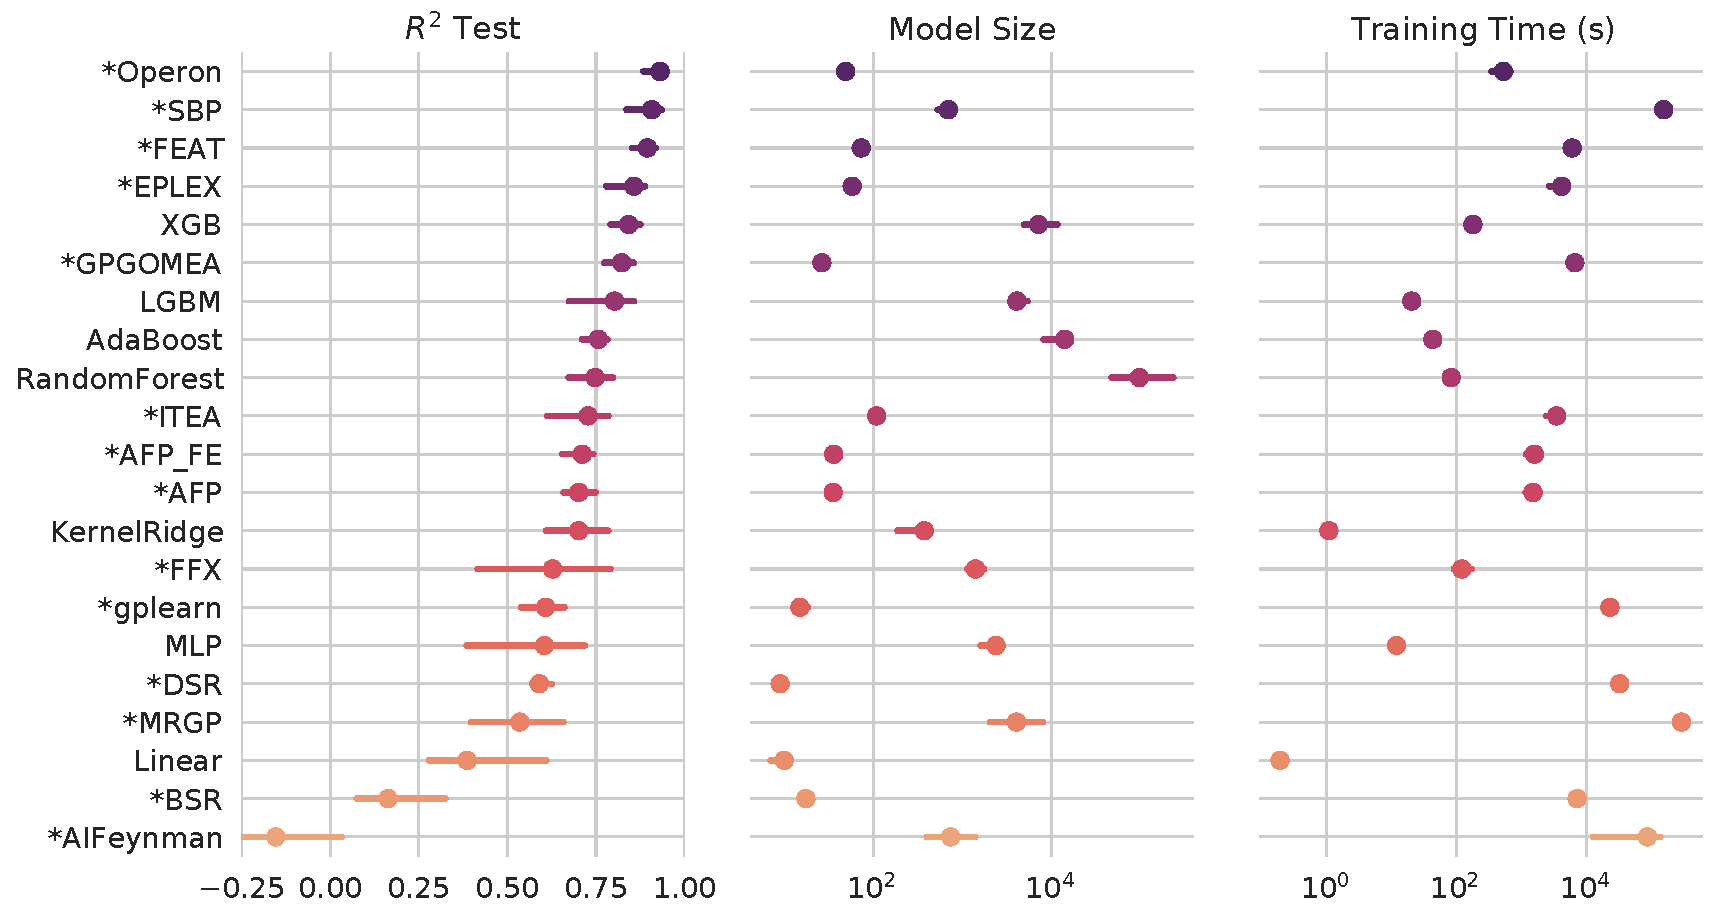
\includegraphics[width=\textwidth]{figs/results_pmlb_r1/pairgrid-pointplot_r2_test_model_size_training-time-(s).pdf}
    \caption{ 
        Results on the black-box regression problems.
        Points indicate the mean of the median test set performance on all problems, and bars show the 95\% confidence interval. 
        Methods marked with an asertisk are SR methods. 
    }
    \label{fig:pmlb_perf}
\end{figure}

% \subsection{Ground-Truth Regression Problems}
% solutions in terms of perfect accuracy, perfect models
% success rates

\begin{figure}
    \centering
    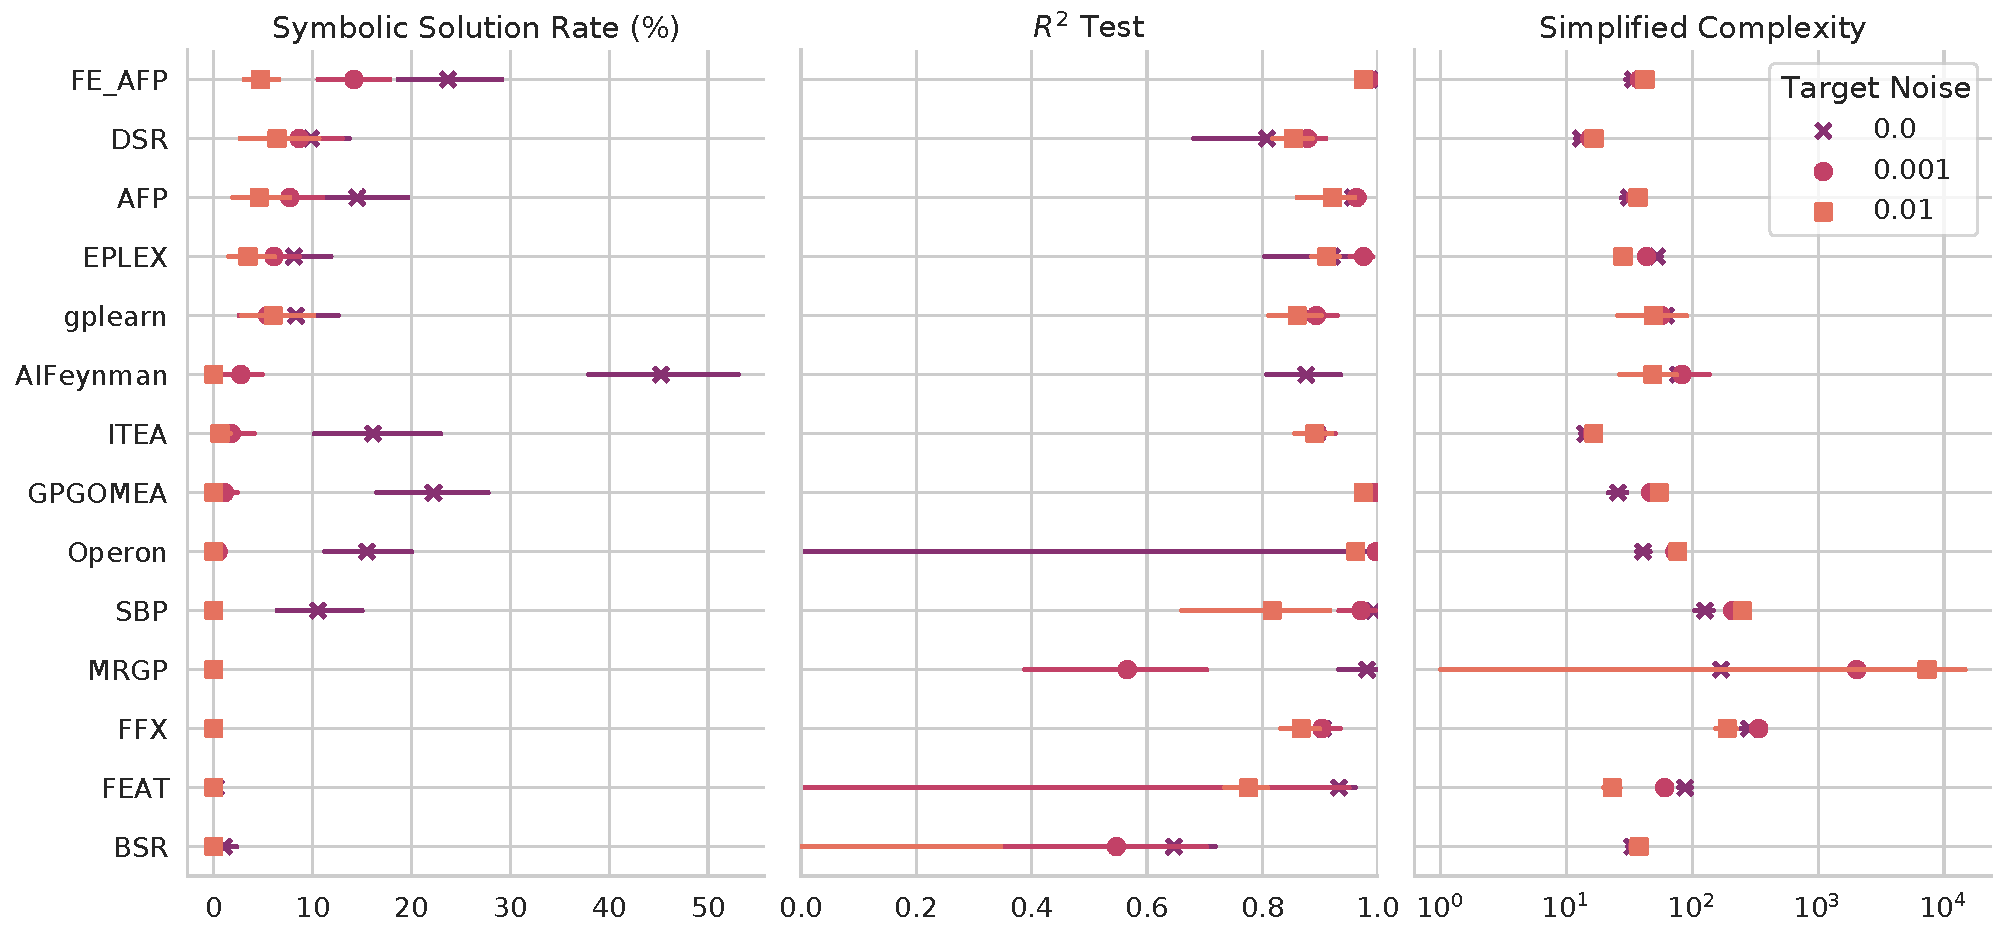
\includegraphics[width=\textwidth]{figs/results_sym_data/pairgrid_symbolic_solution_rate_(pct)_r2_test_simplified_complexity.pdf}
    % \begin{minipage}{0.49\textwidth}
    %     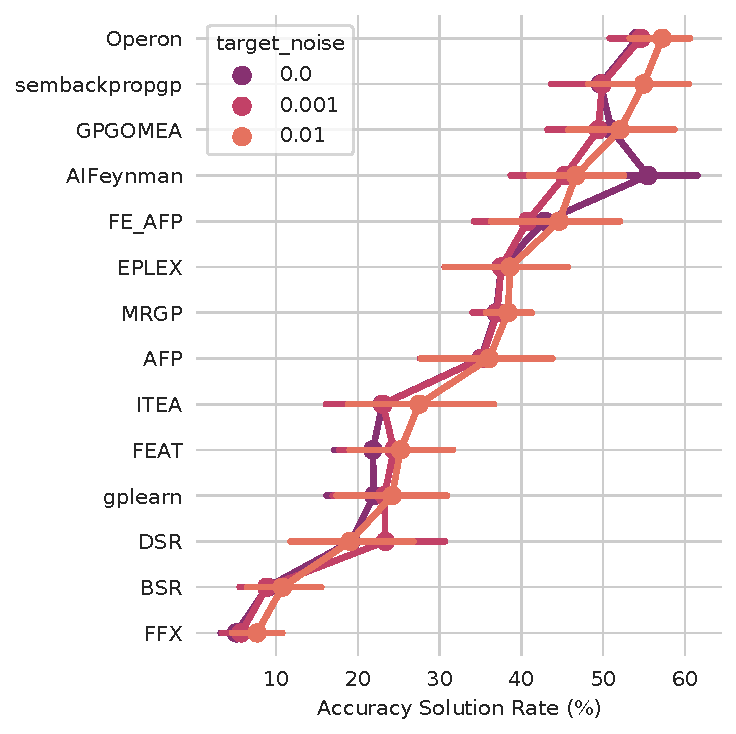
\includegraphics[width=\textwidth]{figs/results_sym_data/cat-pointplot-Accuracy-Solution-Rate-(pct)-by-Algorithm.pdf}
    % \end{minipage}
    % % \hspace{0.01\textwidth}
    % \begin{minipage}{0.49\textwidth}
    %     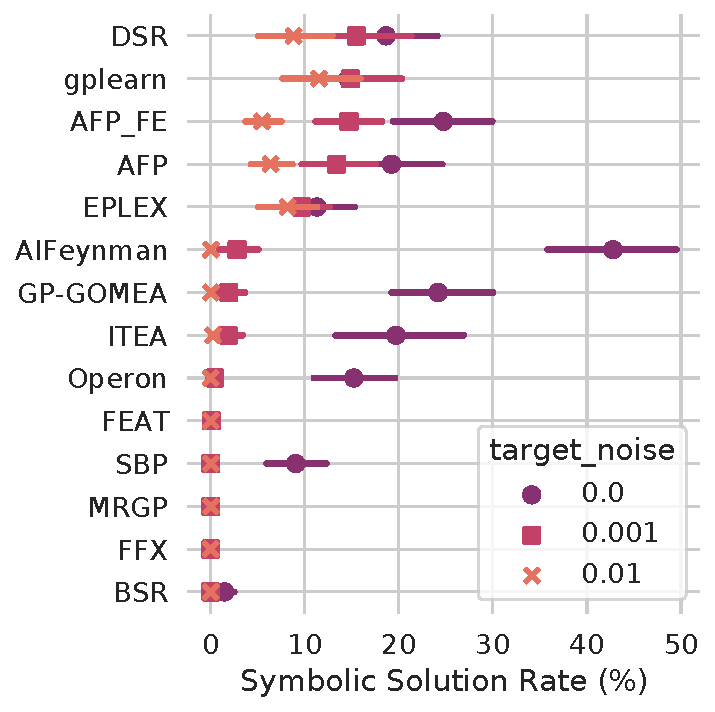
\includegraphics[width=\textwidth]{figs/results_sym_data/cat-pointplot-Symbolic-Solution-Rate-(pct)-by-Algorithm.pdf}
    % \end{minipage}
    \caption{
        Solution rates in terms of perfect accuracy (Left) versus symbolic equivalence (Right) for the Feynman and Strogatz problems. 
        Color indicates level of noise added to the target variable. 
    }
    \label{fig:symbolic_solns}
\end{figure}

% runtime, complexity 
% pareto curves
In Figure~\ref{fig:pareto}, we illustrate the performance of the methods on the black-box problems when accuracy and simplicity are considered simultaneously.
In this case, we prefer methods near the Pareto front of these two objectives, highlighted by the solid line. 
The Pareto front represents the set of solutions that are pure trade-offs between accuracy and simplicity, in the sense that one cannot identify another method that performs as well or better in one of the two objectives without accepting poorer performance in the other.  

% \begin{wrapfigure}{r}{0.6\textwidth}
\begin{figure}
    \centering
    % \begin{minipage}{0.49\textwidth}
    \includegraphics[width=0.6\textwidth]{figs/results_pmlb_r1/pareto_plot_r2_test_rank_model_size_rank.pdf}
    % \end{minipage}
    % \hspace{0.01\textwidth}
    % \begin{minipage}{0.49\textwidth}
    %     \includegraphics[width=\textwidth]{figs/results_sym_data/pareto_plot_r2_test_rank_model_size_rank.pdf}
    % \end{minipage}
    \caption{
        Pareto plot comparing the rankings of SR methods in terms of model size and $R^2$ score on the black-box problems.
        Points are the median ranking across datasets, and the bars represent 95\% confidence intervals. 
        Connecting lines denote the Pareto sets of models. 
        Pareo sets towards the bottom left are the most efficient trade-offs of model size and accuracy. 
    } \label{fig:pareto}
\end{figure}
% \end{wrapfigure}

%%%%%%%%%%%%%%%%%%%%%%%%%%%%%%%%%%%%%%%%%%%%%%%%%%%%%%%%%%%%%%%%%%%%%%%%%%%%%%%%
\section{Discussion and Conclusions}
%%%%%%%%%%%%%%%%%%%%%%%%%%%%%%%%%%%%%%%%%%%%%%%%%%%%%%%%%%%%%%%%%%%%%%%%%%%%%%%%

The main contribution of this paper is providing an objective comparison of SotA symbolic regression methods on a wide range of diverse regression problems.
The methods are analyzed from multiple angles, including their accuracy, running time, but also tolerance of noise, and complexity of provided solutions. 

The popularity of real-life regression problems and need to understand rationale between underlying nature makes our resource a valuable resource in search for interpretable solutions.
%Due to its proprietary nature and incorporation into the DataRobot platform, it is impossible to benchmark Eureqa its performance while controlling for important experimental variables such as computational effort. 



TODO: longer discussion, conclusions etc.

%\begin{itemize}
%    \item directions for improvement in SR
%    \begin{itemize}
%        \item running time
%        \item tolerance to noise
%        \item post-run pruning
%    \end{itemize}
%    \item improvements to benchmarks
%    \begin{itemize}
%        \item feature noise
%        \item add observations of systems with known dynamics. Caveat: real systems and first principles don't always line up, as in metabolic systems~\cite{yeast} and fluid dynamics \cite{lacavaInferenceCompactNonlinear2016}. 
%        \item additional methods: cartesian gp, grammar VAE, etc...
%    \end{itemize}
%\end{itemize}

